% **************************************************
% Document Class Definition
% **************************************************
\documentclass[%
	paper=A4,
	twoside=false,				% onesite or twoside printing
	openright,					% doublepage cleaning ends up right side
	parskip=full,				% spacing value / method for paragraphs
	chapterprefix=true,			% prefix for chapter marks
	11pt,						% font size
	headings=normal,			% size of headings
	bibliography=totoc,			% include bib in toc
	listof=totoc,				% include listof entries in toc
	titlepage=on,				% own page for each title page
	captions=tableabove,		% display table captions above the float env
	draft=false,				% value for draft version
]{scrreprt}
\usepackage[utf8]{inputenc}
\usepackage[english]{babel}

% **************************************************
% Debug LaTeX Information
% **************************************************
%\listfiles

% **************************************************
% Information and Commands for Reuse
% **************************************************
\newcommand{\thesisTitle}{Exposé: Deep Learning Next-Activity Prediction With Cluster-Based Input Data}
\newcommand{\thesisName}{Felix Wolff}
\newcommand{\thesisSubject}{Exposé}
\newcommand{\thesisDate}{August 26, 2015}

\newcommand{\thesisFirstReviewer}{Jane Doe}
\newcommand{\thesisFirstReviewerUniversity}{\protect{Clean Thesis Style University}}
\newcommand{\thesisFirstReviewerDepartment}{Department of Clean Thesis Style}

\newcommand{\thesisSecondReviewer}{John Doe}
\newcommand{\thesisSecondReviewerUniversity}{\protect{Clean Thesis Style University}}
\newcommand{\thesisSecondReviewerDepartment}{Department of Clean Thesis Style}

\newcommand{\thesisFirstSupervisor}{Jane Doe}
\newcommand{\thesisSecondSupervisor}{John Smith}

\newcommand{\thesisUniversity}{\protect{Clean Thesis Style University}}
\newcommand{\thesisUniversityDepartment}{Department of Clean Thesis Style}
\newcommand{\thesisUniversityInstitute}{Institut for Clean Thesis Dev}
\newcommand{\thesisUniversityGroup}{Clean Thesis Group (CTG)}
\newcommand{\thesisUniversityCity}{City}
\newcommand{\thesisUniversityStreetAddress}{Street address}
\newcommand{\thesisUniversityPostalCode}{Postal Code}

% **************************************************
% Load and Configure Packages
% **************************************************

\usepackage[
	figuresep=colon,%
	sansserif=false,%
	hangfigurecaption=false,%
	hangsection=true,%
	hangsubsection=true,%
	colorize=full,%
	colortheme=bluemagenta,%
	bibsys=bibtex,%
	bibfile=bib-refs,%
	bibstyle=alphabetic,%
]{cleanthesis}

\hypersetup{					% setup the hyperref-package options
	pdftitle={\thesisTitle},	% 	- title (PDF meta)
	pdfsubject={\thesisSubject},% 	- subject (PDF meta)
	pdfauthor={\thesisName},	% 	- author (PDF meta)
	plainpages=false,			% 	-
	colorlinks=false,			% 	- colorize links?
	pdfborder={0 0 0},			% 	-
	breaklinks=true,			% 	- allow line break inside links
	bookmarksnumbered=true,		%
	bookmarksopen=true			%
}

% **************************************************
% Document CONTENT
% **************************************************
\begin{document}
\pagenumbering{arabic}
\setcounter{page}{1}
\pagestyle{maincontentstyle}

{\large \thesisName} \\[2mm]
{\LARGE \thesisTitle}

\textbf{Abstract -- Predictive process monitoring is a relatively recent application of predictive analytics in the context of business processes. It is concerned with anticipating the future behaviour of running process instances, based on logs of completed instances. In this thesis we aim at forecasting the next activity in a running case based on event history and data attribute history. The forecasts shall be made via LSTM neural networks trained on clustered input data. One network shall be trained per cluster, while the encoding of past events in the input data shall also be engineered. Performance benchmarks against related recent publications shall complete the thesis.}

\section*{Motivation}
The increasing numbers of knowledge workers brought with it the advent of adaptive case management (ACM) to support them \cite{drucker1999, leclair2009}.
As knowledge workers do not follow a clear and structured approach in their data-intensive work, supporting them via traditional means of business process management is not the best option.
One traditional approach would be the discovery of process models from process logs to analyze and optimize the workflow.
Due to the unstructured nature of knowledge work, an attempt at doing so would likely result in a large \textit{spaghetti model} \cite[ch.14]{Aalst16}.

The course that a case can take is highly dependent on a number of environmental factors, such as data used and produces inside a case \cite{schoenig2018}, and as such can be hard to foresee.
Numerous applications of predictive analytics have proven great accuracy in this context.
These applications are attributed to the domain of predictive process monitoring.
Mostly variables such as remaining cycle time and case outcome have been targeted, but few attempts have been made to target a sequence or the next activity \cite{francescomarino2018, rogge2013}.
This leaves open an opportunity to assist knowledge workers in their daily work without the need for discovering a process model \cite{hauder2014}.
In the long run, one could imagine a recommendation system targeting optimal case outcomes with respect to the individual case state \cite{leclair2009,hauder2014}.

\section*{Background}
\textbf{Predictive process monitoring:}
Process science revolves around managing and optimizing structured procedures, while the broad area of data science covers data mining, algorithmic analysis and predictive analytics. 
Bridging the gap between the two fields is process mining \cite[p.18]{Aalst16}.
It covers the three steps of model discovery, conformance checking and model enhancement \cite{Aalst16}.

These three steps are focused on offline data.
If one would like to avoid a certain process outcome  or e.g. an SLA violation, a guess at future developments requires resorting to online data analysis.
At this step, techniques from the domain of predictive analytics can be employed\footnote{More detail from Marlon Dumas on how these topics fit together: \url{https://www.youtube.com/watch?v=hMQolsRT0K0}}.

Predictive analytics brings together a variety of statistical techniques like data mining, predictive modelling, and machine learning in order to make predictions about future events throught the use of historical data.
In the domain of business processes, statistical or machine learning models are trained with historical process execution logs and \textit{target} a specific piece of data that should be predicted.
This application is called predictive process monitoring and allows answering questions such as \textit{Given the current state of things, will I still meet my SLA?} or \textit{Given the current case state, how long is this case still going to take?}.
The answers to such questions can give case managers the opportunity to intervene if a case takes an unwanted course or might fail to meet KPI requirements.

\textbf{Model training:}
Predictive analytics is a lot about model training, and the rough outline of necessary steps necessary to train a model is listed here:
\begin{enumerate}
    \item Determine the \textit{target} variable, it is the variable that is supposed to be predicted
    \item Preprocess the dataset. This can mean introducing one-hot encodings, normalized values, but also basic data quality assurance such as null value elimination. Feature engineering can also happen at this step.
    \item Partition the dataset into two parts. One part is set aside for model performance verification, as there the actual target variable value is known. This is commonly referred to as the \textit{test set}, while the remainder is called the \textit{training set}.
    \item Train the model on the training set. Models are trained multiple times with different hyper-parameters to find the optimum configuration with respect to prediction accuracy on the test set. Hyper-parameters are model-specific values such as cutoff-thresholds that have impact on model performance.
\end{enumerate}

\textbf{Neural networks with long short-term memory:} An artificial neural network is an example for a machine learning model. It is made up of neurons, similar to its organic counterpart. The network is organized in three types of layers: a single input layer, one or more hidden layers and a single output layer.
The neurons (being mathematical functions), pass their output on to those in the next layer via weighted connections. The weights on these connections are changed as the network is trained \cite{rosenblatt1958}.
Improving this forward-feeding network with backpropagation, i.e. learning from errors, made applications on pattern-detection successful\footnote{Backpropagation can be attributed to many authors, as Schmidhuber blogs: \url{http://people.idsia.ch/~juergen/who-invented-backpropagation.html}}.
Finally, enhancing the network with a way to remember sequences of events allows application on time-series data. The capacity as well as the durability of this memory are purposely limited as to avoid overfitting.
As such, a long short-term memory inside a neural network functions similarly to our human one: we can remember a certain number of things for a short time, but we do forget some of them.
The LSTM feature also equips the network with a remember and a forget capacity \cite{hochreiter1997}.

\textbf{Ensemble learning:} Predictive models vary in complexity, and with it varies their amount of bias and variance.
It can be said that more complex models (such as neural networks or random forests) deliver higher variance and lower bias in their predictions, whereas simpler models (like regressions) exhibit lower variance and higher bias \cite{lessmannBADS}.
This is commonly referred to as the bias-variance tradeoff\footnote{Wikipedia has an exhaustive definition: \url{https://en.wikipedia.org/wiki/Bias\%E2\%80\%93variance_tradeoff}}.
Using several complex models as a basis and training another model using their predictions leverages the diverse strengths of the base models to cancel out their weaknesses \cite{tsoumakas2009}. See figure \ref{fig:ensemble_architecture} for an illustration.
Diversity at the base of such an ensemble can, as so often in life, be the key to good outcomes.
The ensemble strategy (often also referred to as model stacking) should be as simple as possible to avoid further complex rounds of hyper-parameter tuning.

\begin{figure}
    \centering
    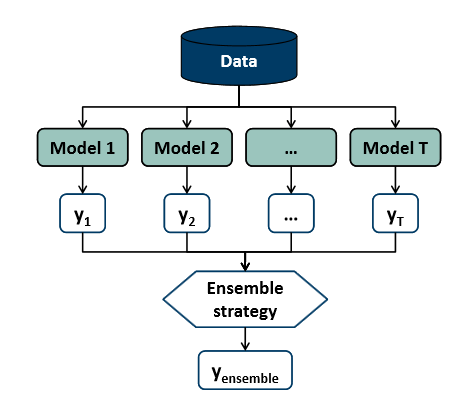
\includegraphics[width=20em]{gfx/ensemble_architecture.png}
    \caption{A generic ensemble architecture, taken from lecture material \cite{lessmannBADS}}
    \label{fig:ensemble_architecture}
\end{figure}

\section*{Related Work}
Hauder et al. mention numerous research challenges in the domain of ACM, among them an active support system for knowledge workers \cite{hauder2014}.
The need for such a system is emphasized by Francescomarino et al. in their literature review, where it has been found that few prediction approaches target the next activity \cite{francescomarino2018}.

An example for how such a system might look like is given by Huber, who has developed a next-step recommendation system serving different case goals.
The system is prototypically implemented into CoCaMa\footnote{CoCaMa is an abbreviation for a project called Collaborative Case Management, which appears to be retired: \url{http://archive.li/uZFnN}}, a prototypical case management application. The system has been evaluated with 25 hand-made case logs.

Building upon each other are the works by Evermann et al. \cite{evermann2016} and Schönig et al. \cite{schoenig2018}.
Evermann et al. have successfully demonstrated the good performance of long-short-term memory (LSTM) neural networks in predicting the next activity.
Their approach did not take into account specific case data attributes however.
How making use of this contextual information can improve the prediction accuracy even more, has been shown by Schönig et al. \cite{schoenig2018}.
Furthermore Schönig et al. have explored data preparation methods for supporting the model during learning.

Similarly, Polato et al. make use of environmental information in their work for improving the prediction of the remaining time of business process instances \cite{polato2014}.

Metzger et al. predict run-time of a case by comparing and combining different prediction models into a model ensemble.
Then, the members of the ensemble are selected based on their predictive performance measures.
This allows taking into account costs of false predictions \cite{metzger2015}.

Francescomarino et al. have performed clustering in the preprocessing phase of model training and prediction.
Having clustered the training data, one model was created and trained for each cluster.
For obtaining a prediction, the optimal cluster for a new data item is found from which the corresponding model is selected.
This approach was evaluated on the accuracy of predicate fulfillment with two different clustering methods (k-means and DBSCAN) and two different prediction models (decision trees and random forests) \cite{francescomarino2015}.
A further evaluation criteria was \textit{earliness}, i.e. at which point in time the correct result could be determined.

\section*{Thesis objective}
In my thesis, I want to investigate the synergies of combining the aforementioned approach of Francescomarino et al. for learning data clustering with LSTM neural networks as per Evermann et al. Case data attributes shall be used during model training and prediction, as Polato et al. \cite{polato2014} and Schönig et al. \cite{schoenig2018} demonstrated their usefulness.

This would contribute to a field of research which is currently being explored and where LSTM networks have been applied successfully on prediction problems with long-term dependencies \cite{evermann2016, tax2017, schoenig2018, graves2005}.

%Furthermore, I want to investigate how much the accuracy of current LSTM approaches is improved if the learning data is clustered.
Furthermore, I want to determine how historical case log data is prepared best for learning, as only Schönig et al. has written a small subsection on this \cite{schoenig2018}.
If time permits, I also want to investigate the potential of ensembles within this context, as they can potentially enlighten the user about the reason for a prediction.
With neural networks it is hard to comprehend the reasons behind a prediction.
Other types of models deliver better comprehensibility.

Throughout the document I will strive to meet recently demanded machine learning paper quality criteria \cite{lipton2018}.

The performance of the combined approaches shall be evaluated against the data from the Business Process Intelligence Challenges (BPIC) 2011, 2012 and 2017 \cite{BPIC2011, BPIC2012, BPIC2017}. This allows for comparison with the results of Francescomarino et al., Evermann et al., Tax et al. and Schönig et al. \cite{francescomarino2018, evermann2016, tax2017, schoenig2018}.
The next steps and an approximate timeframe are shown in the table below:\\[1em]

\begin{table}[!tbh]
    \centering
    \begin{tabular}{l|l}
    Date & Milestone\\
    \hline
    September & Hardware procurement; Reproduction of the results of Schönig et al.\\
    October   & Clustering of data via Francescomarinos method\\
    November  & Hyper-parameter tuning of LSTM neural network\\
              & on clustered training data\\
    December  & Training and benchmarking architecture setup\\
    January   & Benchmarking\\
    February  & Thesis hand-in\\
    March 1st & Defense
    \end{tabular}
    \caption{Approximate timeframe for my work}
    \label{tab:timeframe}
\end{table}

\cleardoublepage
% --------------------------
% Back matter
% --------------------------
{%
\setstretch{1.1}
\renewcommand{\bibfont}{\normalfont\small}
\setlength{\biblabelsep}{0pt}
\setlength{\bibitemsep}{0.5\baselineskip plus 0.5\baselineskip}
\printbibliography[nottype=online]
\printbibliography[heading=subbibliography,title={Webseiten},type=online,prefixnumbers={@}]
}
\end{document}
